{ \large \bfseries 2.Περιγραφή της Σχεδίασης}\\ % title 2


%%Πρώτη φάση

\begin{justify}
\textbf{1\textsuperscript{η} φάση}\\
Στην 1\textsuperscript{η} φάση αρχικά σχεδιάστηκε η 
μονάδα αριθμιτικών και λογικών πράξεων
(\textlatin{ALU}) η οποιά παίρνει σαν είσοδο 
δύο 32\textlatin{bit} τελεστέους και έναν 
4\textlatin{bit} κωδικό πράξης. Ανάλογα με τον κωδικό,
η \textlatin{ALU} βγάζει στην έξοδο το αποτέλεσμα
της πράξης καθώς και 3 διαφορετικά \textlatin{flags}
που επισημαίνουν αν το αποτέλεμσα της πράξης είναι
α) 0, β)έχει κρατούμενο εξόδου 1, γ)έχει υπερχείληση.
Όσον αφορά την υπερχείληση, μπορεί να προκύψει μόνο στην
πρόσθεση και στην αφαίρεση. Στην πρόσθεση, υπάρχει 
υπερχείληση αν και οι δύο προσθετέοι είναι 
ομόσιμοι μεταξύ τους και ετερόσημοι με το αποτέλεσμα, ενώ
στην αφαίρεση έχουμε άν ο μειώτέος είναι είναι θετικός και
ο αφαιρετέος αρνητικός και η διαφορά αρνητική η το ανάποδο.
Για την υλοποίηση των πράξεων χρησιμοποιήθηκαν οι 
βιβλιοθήκες \textlatin{IEEE.NUMERIC\_STD.ALL} και
\textlatin{IEEE.STD\_LOGIC\_SIGNED.ALL} ώστε να 
μην χρειαστεί να υλοποιηθούν από την αρχή τα κυκλώματα
για τις πράξεις.
\end{justify}

\begin{justify}
    Στη συνέχεια σχεδιάστηκαν τα \textlatin{component}
    τα οποία αποτελούν το αρχείο καταχωρητών (\textlatin{register file}). Αρχικά σχεδιάστηκε
    ένας σύγχρονoς καταχωρητς 32\textlatin{bit} 
    με \textlatin{Reset} και \textlatin{WriteEnable}.
    Στη συνέχεια ένας πολυπλέκτης ο οποίος ανάλογα με το
    σήμα \textlatin{sel} (\textlatin{5bit}) επιλέγει ποιά απο τις 32 εισόδος
    θα περάσει στην έξοδο και τέλος ένας αποκωδικοποιητής
    που ανάλογα με το σήμα εισόδου \textlatin{awr} (\textlatin{5bit}) επιλέγει
    ποιό απο τα \textlatin{32bit} της εξόδου θα είναι 1.
\end{justify}

\begin{justify}
    Το αρχείο καταχωρητών περίεχει 2 εισόδους ασύγχρονης
    ανάγνωσης που ελέγχουν 2 πολυπλέκτές και καθορίζουν
    τις εξόδους που θα διαβαστούν, 1 είσοδο σύγχρονης
    εγγραφής που μέσω του αποκωδικοποιητή καθορίζει σε ποιόν
    καταχυρητή θα γράψουμε, την είσοδο των δεδομένων, τα
    σήματα ελέγχου \textlatin{Reset} και \textlatin{WriteEnable}
    και το ρολόι. Χρειάστηκαν 32 καταχωρητές οι 
    οποίοι δημιουργήθηκαν μέσω \textlatin{for-generate}.
    Από αυτούς η τιμή του \textlatin{R0} είναι πάντα 0.
\end{justify}

\begin{justify}
    \textbf{2\textsuperscript{η} φάση}\\
    H 2\textsuperscript{η} φάση αποτελείται από
    4 στάδια. Αρχικά το 1\textsuperscript{ο} στάδιο
    είναι η βαθμίδα ανάκληση εντολων (\textlatin{IF Stage}).
    Σε αυτό το στάδιο διαβάζεται μια εντολή από την μνήμη
    (χρησιμοιόυμε μια \textlatin{Distributed ROM}) και την
    φορτώνουμε σε έναν καταχωρητή, τον \textlatin{Program Counter},
    ο οποίος σε κάθε κύκλο περιέχει την εντολή που εκτελείται
    την συγκεκριμένη χρονική στιγμή. Στον επόμενο κύκλο ο
    \textlatin{PC} προχωράει στην επόμενη εντολή και παίρνει
    την τιμή (\textlatin{{PC}+4}) εκτός αν η εντολή 
    είναι \textlatin{brunch, brunch equal} ή 
    \textlatin{brunch not equal} όπου τότε ο \textlatin{PC}
    παίρνει την τιμή (\textlatin{{PC}+4+Immediate}) και τότε
    η εκτέλεση του προγράμματος μεταφέρεται στην διεύθυνση
    αυτή. Η μνήμη λαμβάνει ως είσοδο τα [11:2] \textlatin{bits}
    της εξόδου του καταχυρητή αφού αυτή είναι οργανωμένη σε 
    \textlatin{words}. Έτσι όσο αυξάνεται ο \textlatin{PC} κατά 4
    η μνήμη θα αυξάνεται κατά 1.
\end{justify}

\begin{justify}
    Το 2\textsuperscript{ο} στάδιο αποτελεί η βαθμίδα
    αποκωδικοποίησης εντολών (\textlatin{DEC Stage}).
    Σε αυτό το στάδιο η εντολή που φορτώνεται από την μνήμη
    αποκωδικοποιείται, με σκοπό την εγγραφή και προσπέλαση της
    στο αρχείο καταχωρητών. Επιπλέον, γίνεται και η κατάλληλη
    επεξεργασία της τιμής \textlatin{Immediate}. Ο καταχωρητής
    ανάγνωσης 1 είναι πάντα ο \textlatin{rs} ενώ ο καταχωρητής
    2 είναι είτε ο \textlatin{rt} είτε ο \textlatin{rd}.
    Ένα πολυπλέκτης καθορίζει ποιός από τους 2 θα περάσει,
    όπου εκεί πρακτικά γίνεται και ο διαχορισμός των \textlatin{R-Type}
    από τις \textlatin{I-Type} εντολές. Ο καταχωρητής εγγραφής
    είναι πάντα ο \textlatin{rd}. Ακόμη η επεξεργασία του
    \textlatin{Immediate} γίνεται στην μονάδα \textlatin{"Cloud"}
    όπου ανάλογα με την τιμή του σήματος \textlatin{CloudControl}
    γίνεται \textlatin{1.Zero Fill}, \textlatin{2.Sign Extend},
    \textlatin{3.Zero Fill \& Shift} και \textlatin{4.Sign Extend \& Shift 2}.
    Tέλος, η είσαγωγή των δεδομένων προς εγγραφή στο 
    \textlatin{Register File} επιλέγεται μέσω ενός άλλου
    πολυπλέκτη να είναι είτε από την μνήμη \textlatin{RAM}
    σε περίπτωση των εντολών \textlatin{load} και \textlatin{store}
    είτε απο την έξοδο της \textlatin{ALU} στις υπόλοιπες εντολές.
\end{justify}

\begin{justify}
    Το 3\textsuperscript{ο} στάδιο είναι η βαθμίδα εκτέλεσης
    εντολών (\textlatin{EX Stage}). Σε αυτό το στάδιο γίνεται
    η εκτέλεση της εντολής και ο υπολογισμός του αποτελέσματος της
    \textlatin{ALU}. Το 1\textsuperscript{ο} σήμα εισόδου της
    αποτελούν τα δεδομένα ανάγνωσης του καταχωρητή 1(έξοδος απο
    \textlatin{Register File}) και το 2\textsuperscript{ο}
    μέσω ενός πολυπλέκτη είναι είτε τα δεδομένα ανάγνωσης του
    καταχωρητή 2 είτε το επεξεργασμένο \textlatin{Immediate}.
\end{justify}

\begin{justify}
    Το 4\textsuperscript{ο} και τελευταίο στάδιο αποτελεί
    η βαθμίδα πρόσβασης μνήμης (\textlatin{MEM Stage}).
    Σε αυτό το στάδιο υλοποιήθηκε μια μνήμη \textlatin{RAM}
    1024 θέσεων των 32\textlatin{bit}. Η μνήμη είναι
    \textlatin{Read First} και έχει μια θύρα ανάγνωσης και εγγραφής.
\end{justify}

\begin{justify}
    Τέλος για την υλοποίηση της εντολής \textlatin{load byte}
    έχει δημιουργήθεί ένα \textlatin{LS Stage} το οποίο παίρνει
    σαν είσοδο την έξοδο της μνήμης \textlatin{RAM} και
    μέσω ενός πολυπλέκτη επιλέγει εάν θα βγει αυτούσια στην έξοδο 
    είτε αν ,στην περίπτωση της εντολής \textlatin{load byte},
    γίνει \textlatin{Zero Fill} στα \textlatin{bit} [31:8].

\end{justify}

\newpage

\begin{justify}
    \textbf{3\textsuperscript{η} φάση}\\
    Στην 3\textsuperscript{η} φάση ενώθηκαν τα 4 στάδια
    και υλοποιήθηκε το \textlatin{DATAPATH} το οποίο 
    πρακτικά είναι υπεύθυνο για να πραγματοποιήσει όλες τις
    λειτουργίες του επεξεργστή, ανάλογα με τις εντολές που 
    εισάγονται.\\
\end{justify}

\begin{figure}[h]
    \raggedright
    \hspace{-1cm}
    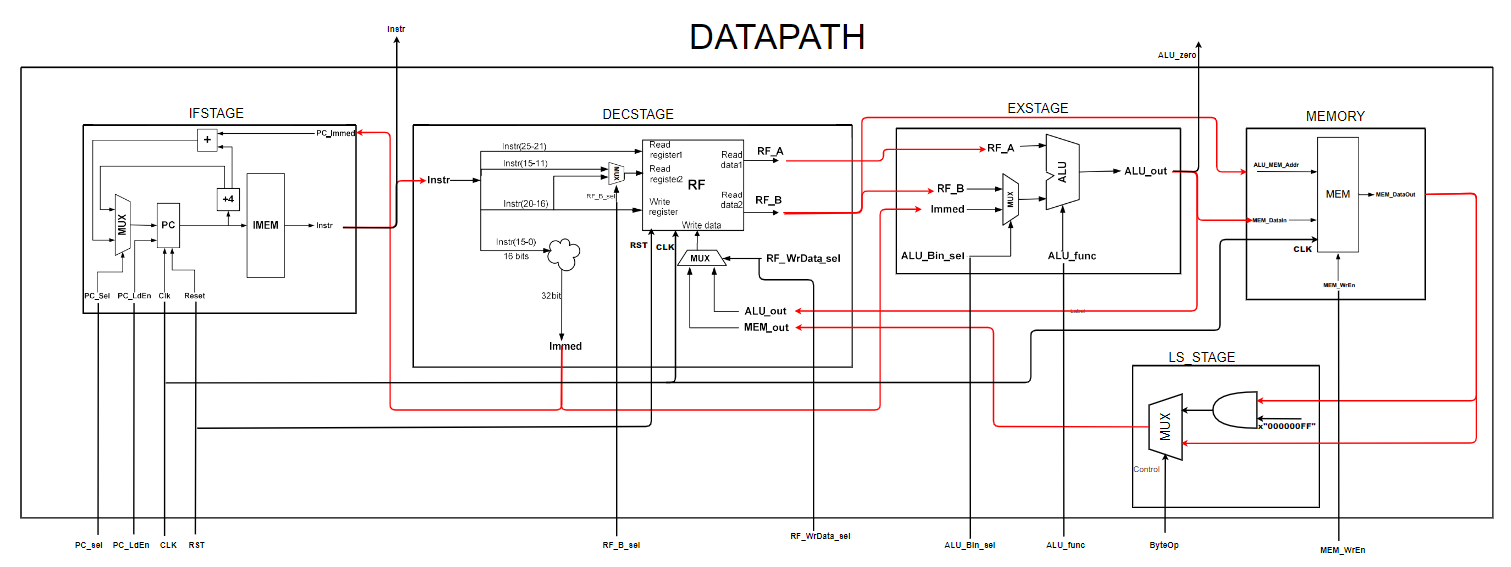
\includegraphics[width=1.1\textwidth]{Images/DATAPATH_Lab1.png} % Adjust width as needed
\end{figure}

\begin{justify}
    Στην συνέχεια δημιουργήθηκε το \textlatin{CONTROL} το οποίο
    είναι υπεύθυνο να στέλνει τα κατάλληλα σήματα ελέγχου στο
    \textlatin{DATAPATH} ανάλογα με την εντολή που εκτελείται.
    Παίρνει σαν εισόδους ένα ασύγχρονο \textlatin{Reset} καθώς και
    το \textlatin{flag Zero} της \textlatin{ALU} το οποίο
    χρησιμοποιείται στις εντολές διακλαδώσεων \textlatin{brunch}
    και παράγει εξόδους για όλα τα σήματα εισόδου του
    \textlatin{DATAPATH}.    
\end{justify}

\begin{justify}
    Το \textlatin{DATAPATH} και το \textlatin{CONTROL} ενώθηκαν
    σε ένα \textlatin{Top Level} αρχείο \textlatin{PROCESSOR}
    το οποίο τρέχει και επιβεβαιώνει την ορθή λειτουργία του επεξεργστή.
    Δεν έχει εισόδους και εξόδους πέρα από το \textlatin{Reset}
    και το ρολόι.
\end{justify}

\begin{figure}[h]
    \centering
    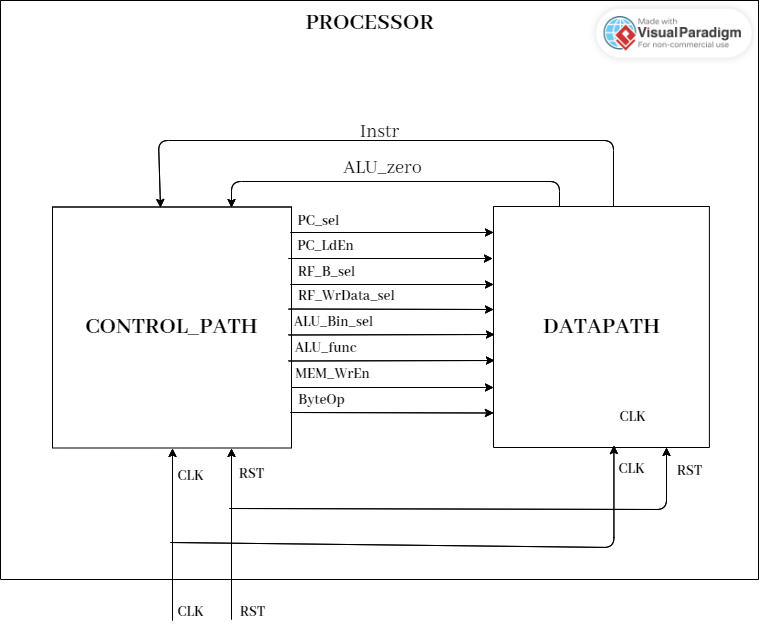
\includegraphics[width=0.6\textwidth]{Images/CDPATH.png} % Adjust width as needed
\end{figure}





